\chapter{Chemical Reactions}

\section{Chemical Reactions}

\begin{wrapfigure}{l}{3in}
\noindent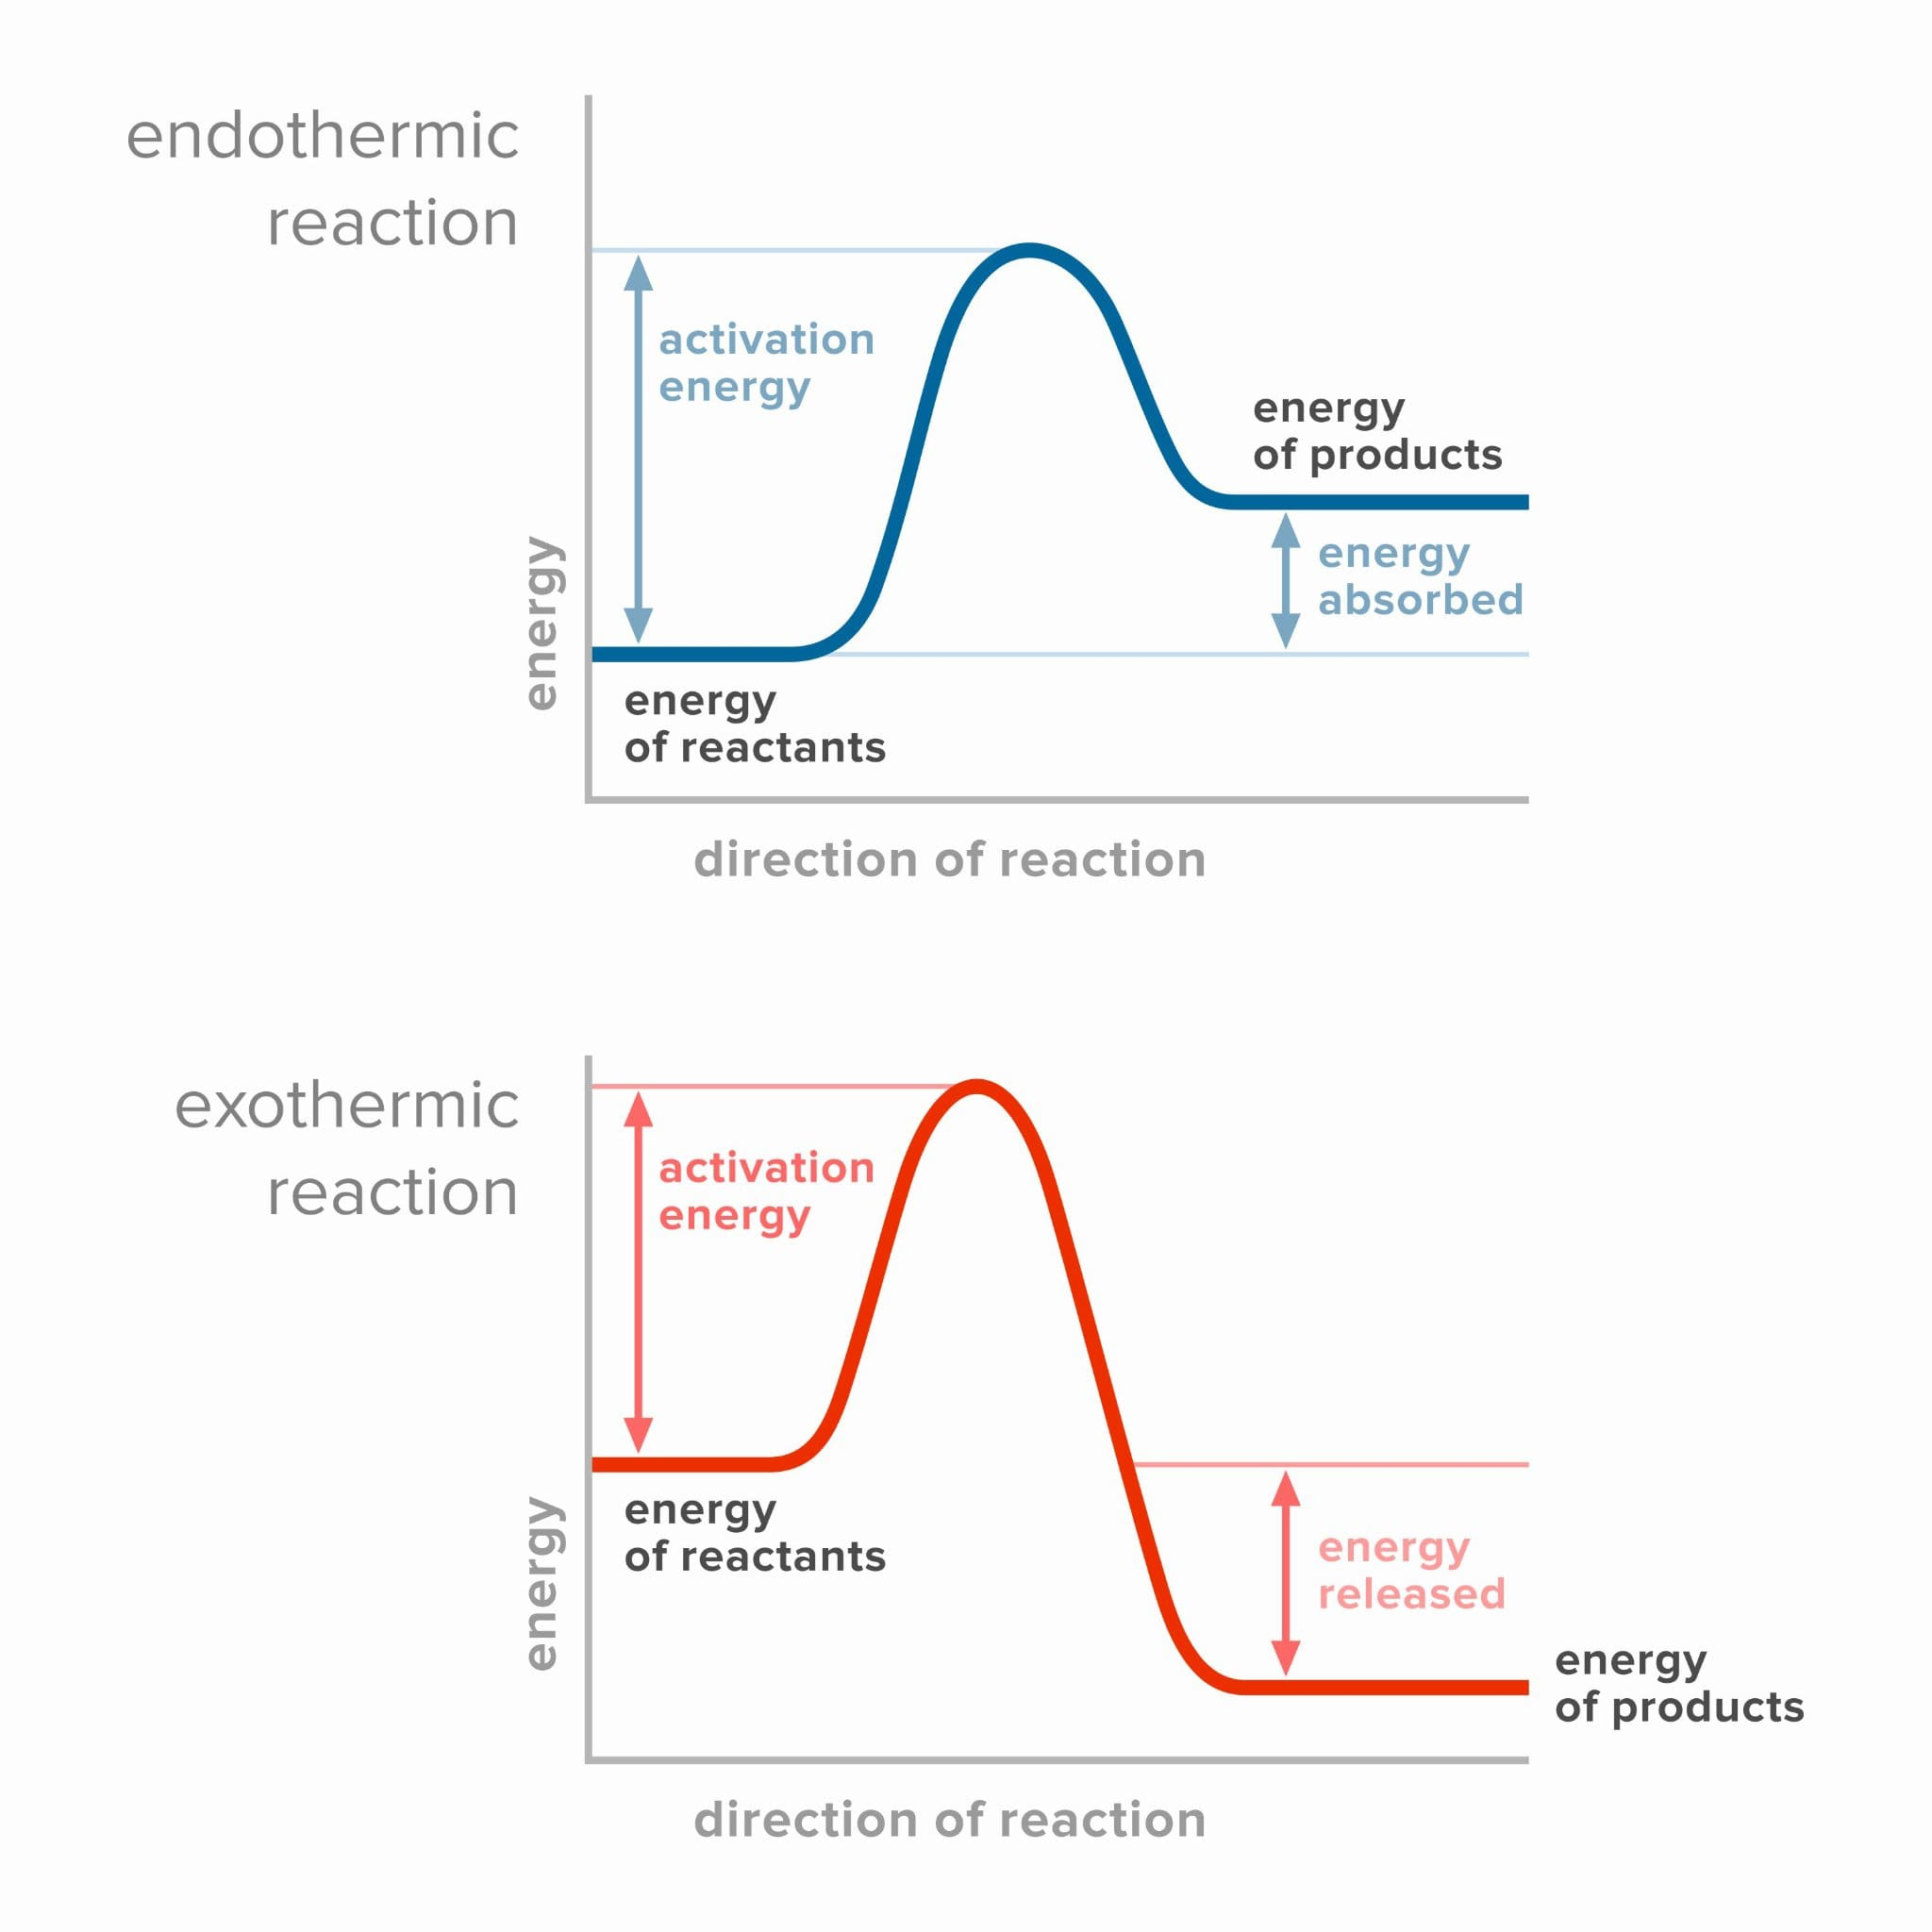
\includegraphics[width=3in]{exo_endo_diagrams.png}
\caption{}
\label{fig:exo_endo_diagrams}
\end{wrapfigure}

Sometimes two hydrogen atoms form a molecule ($H_2$). Sometimes two oxygen
atoms form a molecule ($O_2$). If you mix these together and light a match,
they will rearrange themselves into water molecules. This is called a \textit{
chemical reaction}. In any chemical reaction, the atoms are rearranged into new
molecules.\index{chemical reaction}

Some chemical reactions (like the burning of hydrogen gas described above) are
\textit{exothermic} --- that is, they give off energy. Burning hydrogen gas
happens quickly and gives off a lot of energy. If you have enough, it will make
quite an explosion! \index{exothermic}

Other chemical reactions are \textit{endothermic} --- they consume energy.
Photosynthesis, the process by which plants consume energy from the sun to make
sugar from $CO_2$ and $H_2O$ requires an endothermic chemical reaction.\index{endothermic}

Examine the diagrams in figure \ref{fig:exo_endo_diagrams}. The $x$-axis 
represents time - time passes as wemove from left to right across the diagram. 
At the far left, the energy of the reactants (the ingredients that go into the 
reaction) is shown. At the far right, the energy of the products (what is made in 
the chemical reaction) is shown. The red diagrams shows an exothermic reaction: 
the products (what is made) have less energy than the reactants (the "ingredients"
that start the reaction). Since energy is never created or destroyed, where did 
the energy go? It is released as heat. So, exothermic reactions release heat.

Now, look at the endothermic reaction diagram (the blue one). Based on the
relative energies of the reactants and products, do you expect and endothermic
reaction to release or absorb heat? Absorb! Since the products have more
energy, they must have absorbed energy, in the form of heat, from the surroundings.
%FIXME - idea? maybe reverse the order of the paragraphs since endothermic is first in the figure?
What does this look and feel like in real life? If an exothermic reaction were
happening in a glass beaker, you would feel warmth if you held the beaker. The
heat is leaving the beaker and entering your hand, which feels warm. What
about an endothermic reaction? Many students think that since an endothermic
reaction absorbs heat, it must be getting hot. This is incorrect:
\textit{exothermic} reactions feel hot. If an endothermic reaction were
happening in a beaker and you touched the beaker, it would feel \textbf{cold}.
Why? Well, if the reaction is absorbing heat, then heat must be leaving it
surroundings (your hand) and entering the reaction (this heat energy is turned
into chemical energy that is stored in the new chemical bonds that are
forming). So your hand feels cold. %fixme: models showing flow of heat in/out of system for chemical reactions.

%FIXME great place to talk about endergonic and exergonic reactions